% 第 17 题四棱锥 P-ABCD：顶点坐标按固定源 PDF 矢量路径端点换算（1 pt → 0.04 cm）。
% 实线 5 段：AD、DP、CD、CP、AP；虚线 4 段：AB、BC、BD、BP（B 为虚线汇聚点，BD 为底面对角线勿漏）。
% 全图唯一相交处：虚线 BC 与实线 PD（虚线在交点两侧断开、实线连续）——先画虚线后画实线即得。
% PA 竖直且与 AD 等长；BC ∥ AD（图面同高）且 BC = AD/2（投影保持）；本卷图中无 E 点。
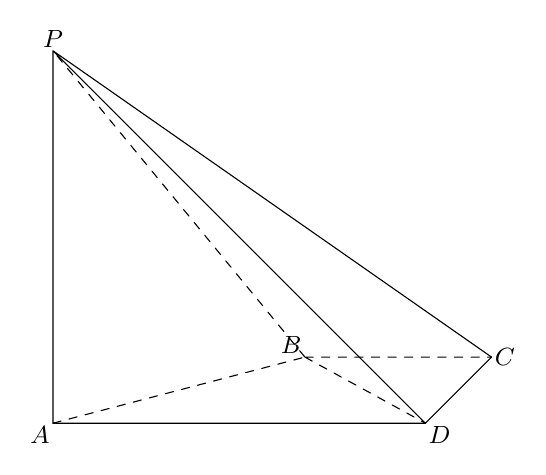
\begin{tikzpicture}[line cap=round,line join=round,font=\small]
\coordinate (P) at (0,4.73);
\coordinate (A) at (0,0);
\coordinate (B) at (3.20,0.84);
\coordinate (C) at (5.57,0.84);
\coordinate (D) at (4.73,0);
% 虚线先画
\draw[dashed] (A)--(B) (B)--(C) (B)--(D) (B)--(P);
% 实线后画（压住虚线交叉处，与原图一致）
\draw (A)--(D) (D)--(P) (C)--(D) (C)--(P) (A)--(P);
\node[above,inner sep=1pt] at (P) {$P$};
\node[below left,inner sep=1pt] at (A) {$A$};
\node[above left,inner sep=1pt] at (B) {$B$};
\node[right,inner sep=1pt] at (C) {$C$};
\node[below right,inner sep=1pt] at (D) {$D$};
\end{tikzpicture}
